	
	\subsection{Дифференциальные формы}	
	
	Начнём с определения дифференциальных форм. 

	\begin{definition} 
		\emph{Дифференциальная 1-форма} на $\R^n$~--- это объект вида 
		\[
			\omega = \sum_{i = 1}^{n} f_i(x) \mathrm{d}x_i, \quad x = (x_1, \ldots, x_n) \in \R^n, \ f_i \in C^{\infty}(\R^n),
		\]
		где $\mathrm{d}x_i$~--- <<значки>>, которые пока что ничего не означают и преобразуются по формальным правилам. 
	\end{definition}

	Соотвественно, каждой точке $x$ $\omega_{x}$~--- просто элемент $\R$-векторного пространства, натянутого на $\mathrm{d}x_1, \ldots, \mathrm{d}x_n$. Пространство 1-форм имеет естественную структуру $C^{\infty}(\R^n)$-модуля, его мы будем обозначать как $\Omega^{1}(\R^n)$. 

	Если $g\colon \R^k \to \R^n$ (а координаты в $\R^k$~--- это $y_1, \ldots, y_k$)~--- гладкое отображение, то $x_i = x_i(y_1, \ldots, y_k)$ и мы будем полагать, что в таком случае $\mathrm{d}x_i$ изменяются вот по таким правилам: 
	\[
		\mathrm{d}x_i = \sum_{j = 1}^{k} \frac{\partial x_i}{\partial y_j} \mathrm{d}y_{j}.
	\]
	Тогда для $\omega = \sum f_i \mathrm{d}x_i$ её \emph{пулл-бэк} или \emph{pull-back} вдоль $g$ мы определим, как 
	\[
		g^{*}(\omega) \eqdef \sum_{i = 1}^{n} f_{i} \sum_{j = 1}^{k} \frac{\partial x_i}{\partial y_{j}} \mathrm{d}y_{j}.
	\]

	Соотвественно, для пути $\gamma\colon [0,1] \to \R^n$ мы можем интгерал формы $\omega$ вдоль $\gamma$ следующим образом: 
	\[
		\int\limits_{\gamma} \omega \eqdef \int\limits_{[0, 1]} \gamma^{*}\omega = \int\limits_{[0, 1]} \sum f_{i} \cdot \gamma_{i}' \mathrm{d} t= \int\limits_{[0, 1]} \gamma' \cdot (f_1, \ldots, f_n) \mathrm{d}t
	\]

	\begin{definition} 
		Дифференциальная $k$-форма на $\R^n$~--- это формальная линейная комбинация 
		\[
			\omega = \sum_{|I| = k} f_{I}(x)\  \mathrm{d}x_{i_{1}} \wedge \mathrm{d} x_{i_{2}} \wedge \ldots \wedge \mathrm{d}x_{i_{k}}, \quad f_{I} \in C^{\infty}(\R^n)
		\]
		где $\wedge$-произведение как и обычно антисимметрично: $\mathrm{d}x_i \wedge \mathrm{d}x_{j} = - \mathrm{d}x_{j} \wedge \mathrm{d}x_{i}$.

		Пространство $k$-форм мы будем обозначать, как $\Omega^k(\R^n)$.
	\end{definition}

	Из соображений антисимметричности внешнего произведения, достаточно полагать наборы монотонными, то есть $i_{1} < i_{2} < \ldots < i_{k}$. 

	Опять же, если есть отображение $\gamma\colon [0, 1]^k \to \R^n$ и $k$-форма $\omega = \sum_{|I| = k} f_{I} \ \mathrm{d}x_{i_{1}} \wedge \ldots \mathrm{d}x_{i_{k}}$, то можно определить 
	\[
		\int\limits_{\gamma} \omega \eqdef \int\limits_{[0, 1]^k} \gamma^* \omega, \text{ где } \gamma^{*}(\mathrm{d}x_1 \wedge \ldots \wedge \mathrm{d}x_k) = \gamma^*(\mathrm{d}x_1) \wedge \ldots \wedge \gamma^*(\mathrm{d}x_k).
	\]

	\begin{example}
		Пусть $\gamma\colon [0, 1]^2 \to \R^3, \ \gamma(t_1, t_2) = (t_1, t_2, t_1 t_2)$, в $[0, 1]^2$ у нас координаты $(t_1, t_2)$, а в $\R^3$ у нас координаты $(x, y, z)$.

		Рассмотрим форму $\omega = xy \mathrm{d}y \wedge \mathrm{d}z$, её пулл-бэк: 
		\[
			\gamma^*(\omega) = t_1 t_2 \mathrm{d}t_2 \wedge \mathrm{d}(t_1 t_2)
		\]
		\[
			d(t_1 t_2) = \frac{\partial(t_1 t_2) }{\partial t_1} \mathrm{d}t_1 + \frac{\partial(t_1 t_2) }{\partial t_2} \mathrm{d}t_2 = t_{2} \mathrm{d}t_1 + t_{1}\mathrm{d}t_2 \rightsquigarrow \gamma^*(\omega) = t_1 t_2 \mathrm{d}t_2 \wedge (t_2 \mathrm{d}t_1 + t_1 \mathrm{d}t_2) = -t_1 t_2^2 \mathrm{d}t_1 \wedge \mathrm{d}t_2.
		\]
		
	\end{example}

	\begin{remark}
		Из определения мы видим, что пулл-бэк $k$-формы~--- $k$-форма. 
	\end{remark}

	В частности, из нашей игры с обозначениями сразу следует, что 
	\[
		\int\limits_{[0, 1]^k} f\ \mathrm{d}x_{1} \wedge \ldots \wedge \mathrm{d}x_{k} = \int\limits_{[0, 1]^k} f \  \mathrm{d}x_{1}  \ldots \mathrm{d}x_{k}
	\]

	Абстрактно всё озвученное выше можно воспринимать следующим образом:  $k$~--- формы~--- это сечения $\Lambda^k T^* \R^n$ (и, с формальной точки зрения, все выписанные выше формулы будут абсолютно такими же). 


	Теперь рассмотрим $\omega \in \Omega^1(\R^n)$, в каждой точке $x \in \R^n$ это 
	\[
		\omega_x = \sum_{i} a_{i} \mathrm{d}x_{i}.
	\]

	Тогда значок $\mathrm{d}x_i$ можно понимать, как функционал на $T_{x}\R^n$, действующий как 
	\[
		v \in T_{x}\R^n, \ v = (v_1, \ldots, v_n) \quad \mathrm{d}x_i(v_1, \ldots, v_n) = v_i. 
	\]
	Тогда $\sum_{i} a_{i} \mathrm{d}x_i$~--- тоже функционал на $T_{x}\R^n$. Кроме того, если же $V$~--- векторное поле на $\R^n$, то тогда $\mathrm{d}x_i(v)$~--- функция на $\R^n$ (в каждой точке вычисляющая $v(x)_{i}$).

	Теперь определим \bf{внешний дифференциал}. Пусть $\omega \in \Omega^k(\R^n)$, $\omega = \sum_{|I| = k} f_{I} \mathrm{d}x_{I}$, тогда $d\omega$ определяется, как 
	\[
		\mathrm{d}\omega = \sum_{|I| = k} \sum_{i = 1}^{n} \frac{\partial f_{I}}{\partial x_{i}} \mathrm{d}x_i \wedge \mathrm{d}x_{I} \in \Omega^{k + 1}(\R^n). 
	\]

	Нетрудно видеть, что внешний дифференциал~--- это линейное отображение 
	\[
		\mathrm{d} \colon \Omega^k(\R^n) \to \Omega^{k + 1}(\R^n).
	\]

	Кроме того, если $f \in C^{\infty}(\R^n)$, то справедлива формула 
	\[
		\mathrm{d}(f\cdot \omega) = \mathrm{d}f \wedge \omega + f \mathrm{d}\omega.
	\]

	\begin{homework} Внешний дифференциал коммутирует с пулл-бэком, то есть если $g \in \R^m \to \R^n$, а $\omega \in \Omega^k(\R^n)$, то 
	\[
		\mathrm{d}g^*(\omega) = g^{*}\mathrm{d}\omega. 
	\]
	\end{homework}

	\begin{definition} 
		Если $\mathrm{d} \omega = 0$, то форму $\omega$ мы будем называть \emph{замкнутой}. Если $\omega = \mathrm{d}\alpha$ для некоторой $\alpha$, то форму $\omega$ мы будем называть \emph{точной}. 
	\end{definition}

	\begin{lemma} 
		$d^{2} = 0$ (т.е., как отображение $\Omega^k(\R^n) \to \Omega^{k + 2}(\R^n)$ это умножение на 0). 
	\end{lemma}
	\begin{proof}
		Пусть $\omega = \sum_{I} f_{I} \mathrm{d}x_I$. В силу линейности достаточно проверить утверждение для $f_I \mathrm{d}x_{I}$. 

		\[ 
			f_{I} \mathrm{d}x_I \mapsto \sum_{i} \frac{\partial f}{\partial x_i} \mathrm{d}x_i \wedge \mathrm{d}x_{I} \mapsto \sum_{j} \sum_{i} \frac{\partial f}{\partial x_j \partial x_i} x_j \wedge x_i \wedge x_I.
		\]
		Остаётся заметить, что каждому слагаемому $\ldots \mathrm{d}x_j \wedge \mathrm{d}x_i $ будет соотвествовать слагаемое $- \mathrm{d}_i \wedge \mathrm{d}x_j$ (и они сократятся). 
	\end{proof}

	Это означает, что $\mathrm{d}$~--- дифференциал в смысле гомологической алгебры, а 
	\[
		\Omega^0(\R^n) \xrightarrow{d} \Omega^{1}(\R^n) \to \ldots \xrightarrow{d} \Omega^n(\R^n) \to \ldots
	\]
	это \emph{дифференциальный комплекс}. 

	\begin{theorem}[Стокс] 
		Пусть $c$~--- $k$-мерная сингулярная цепь, а $\omega$~--- $(k - 1)$-форма, тогда 
		\[
			\int\limits_{c} \mathrm{d}\omega = \int\limits_{\partial c} \omega.
		\]
	\end{theorem}
	\begin{proof} Вот же оно:
		\begin{center}
			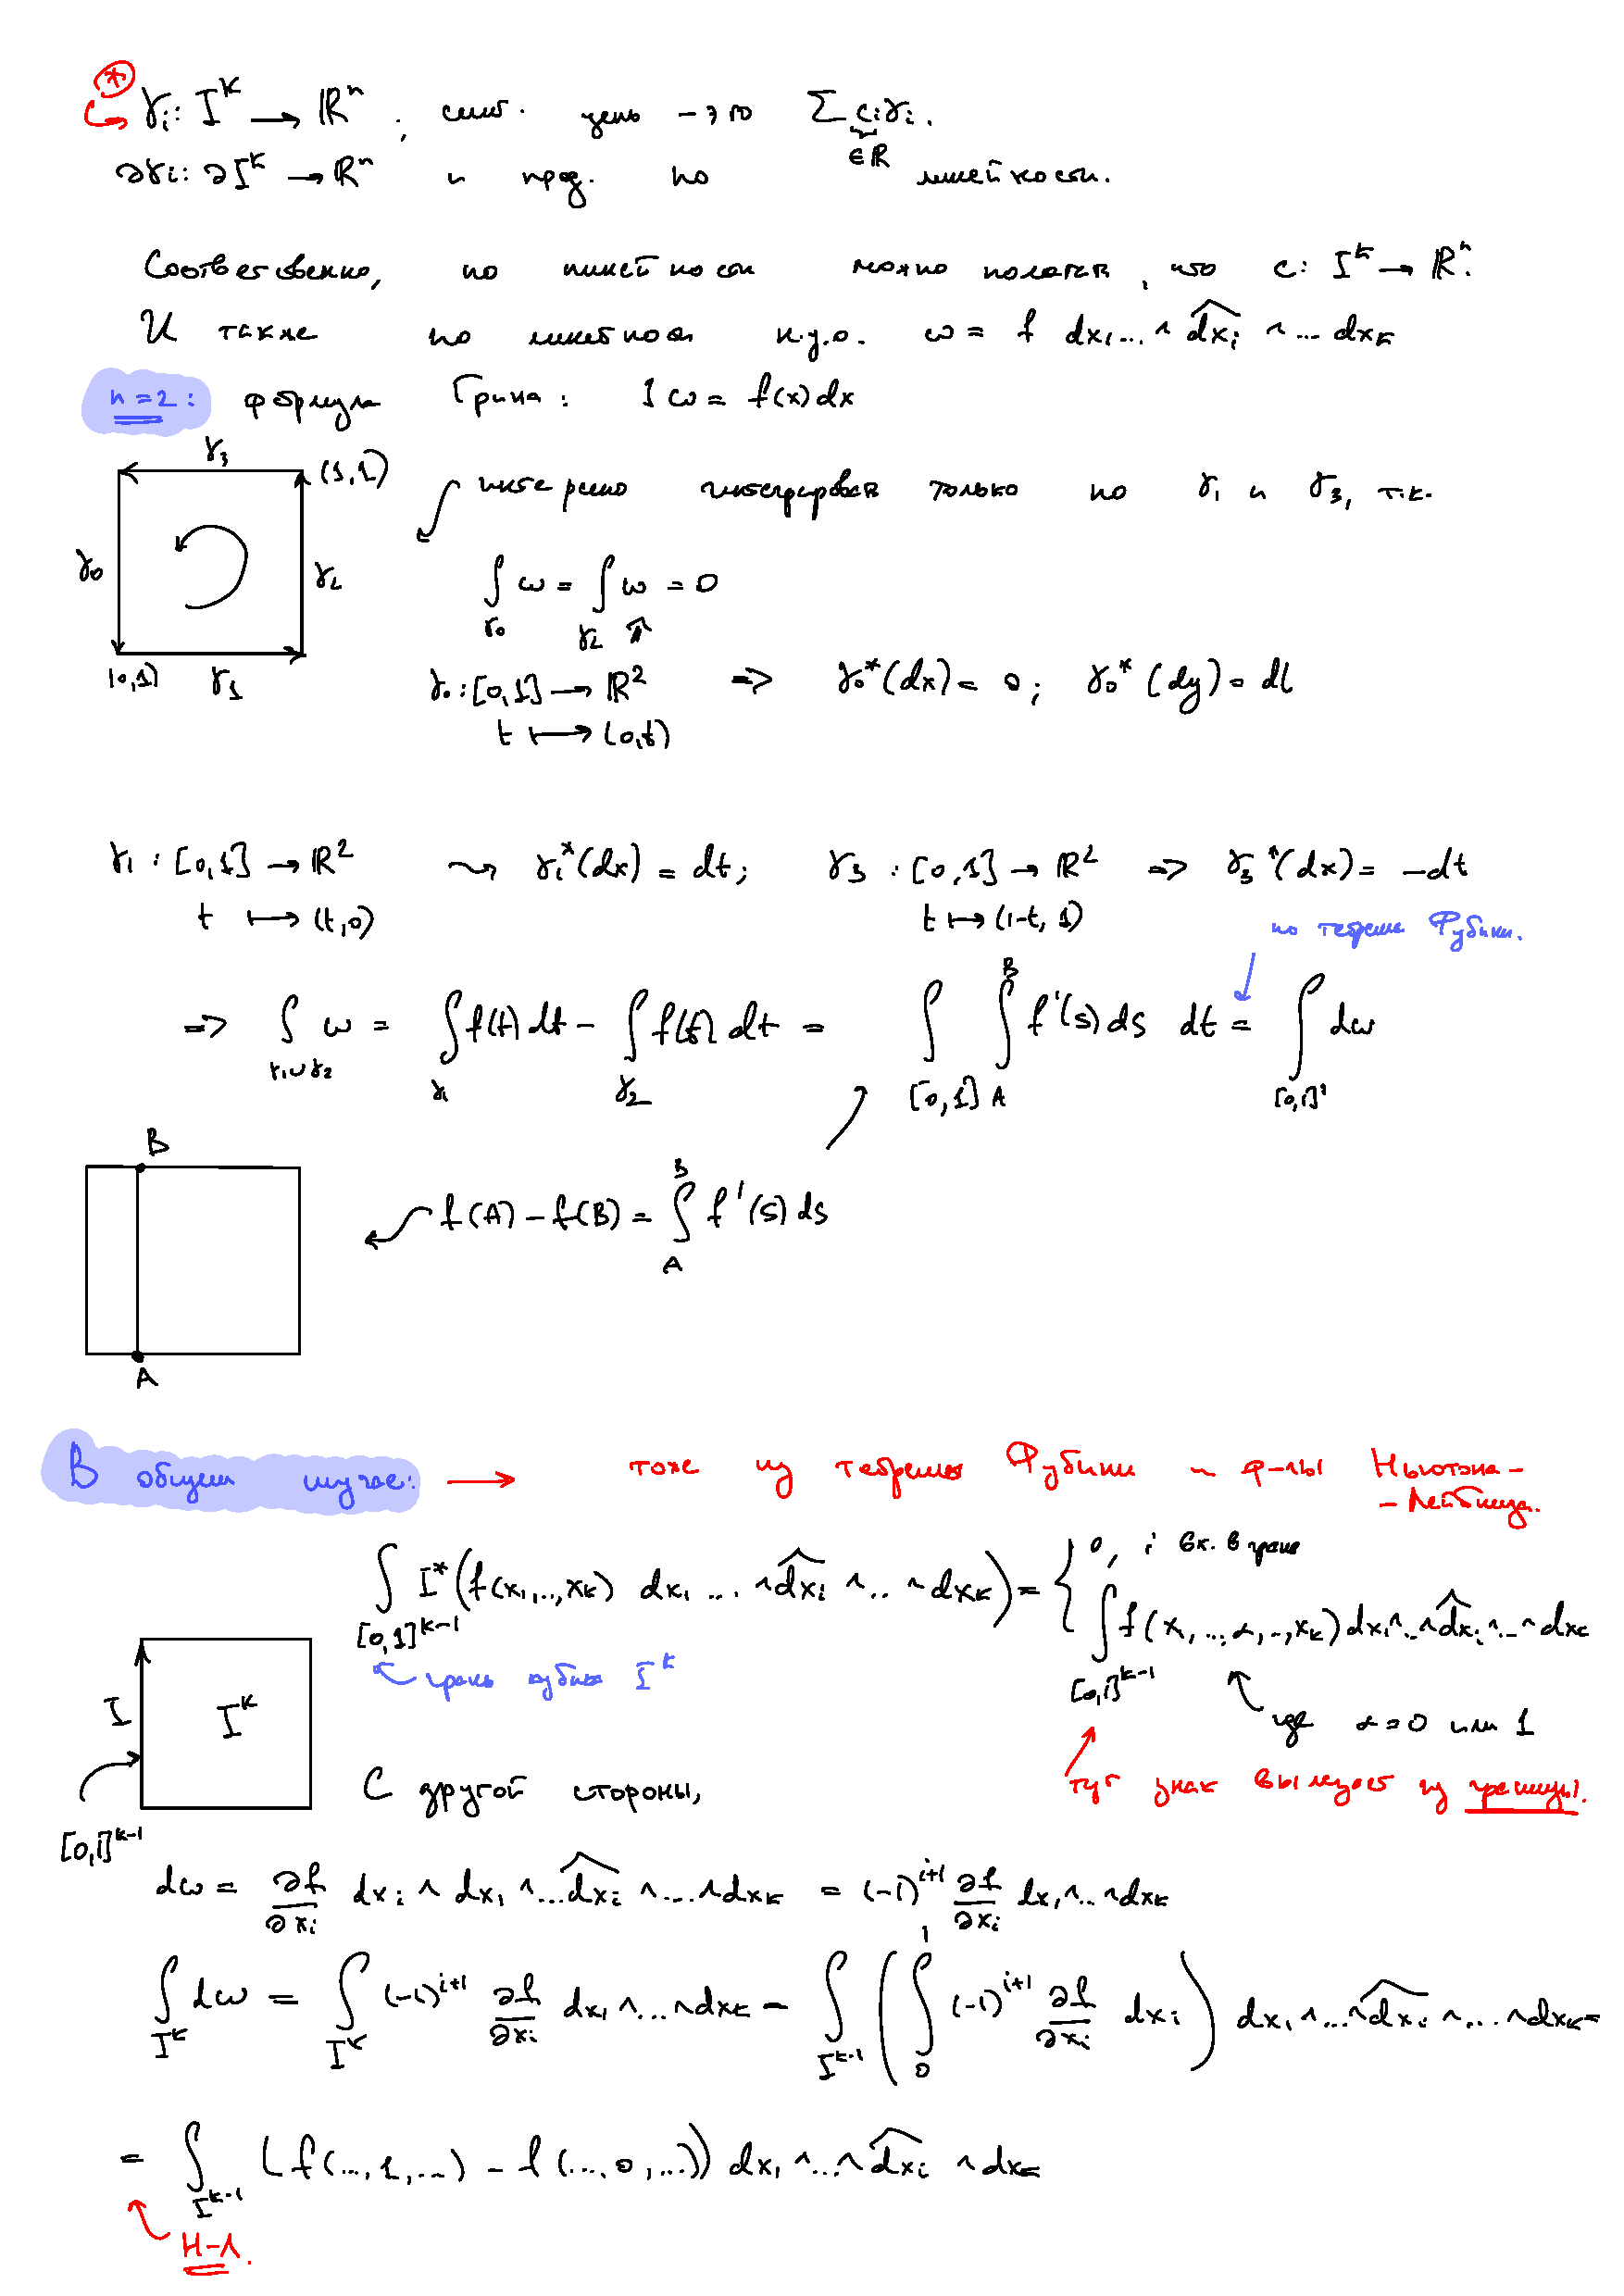
\includegraphics[scale = 0.55]{lectures/7/pictures/Stonks_formula.pdf}
		\end{center}
	\end{proof}

		\begin{example}
		Посмотрим на дифференциальные формы на $\R^3$. 

		\begin{itemize}
			\item $\Omega^{0}(\R^3) = C^{\infty}(\R^3)$.

			\item $\Omega^1(\R^3) = \{ f_1 \mathrm{d}x + f_2 \mathrm{d}y + f_3 \mathrm{d}z, \ f_i \in C^{\infty}(\R^3) \}$.

			\item $\Omega^{2}(\R^3) = \{ f_1 \mathrm{d}x \wedge \mathrm{d}y + f_2 \mathrm{d}y \wedge \mathrm{d}z + f_3 \mathrm{d}z \wedge dx, \ f_i \in C^{\infty}(\R^3) \}$.

			\item $\Omega^{3}(\R^3) = \{ f \mathrm{d}x \wedge \mathrm{d}y \wedge \mathrm{d}z, \ f \in C^{\infty}(\R^3) \} $.
		\end{itemize}

		Видно, что у нас есть отождествления $C^{\infty}(\R^3) \cong \Omega^0(\R^3) \cong \Omega^{3}(\R^3)$.

		Кроме того, как мы помним, гладкие векторные поля на $\R^3$~--- это 
		\[
			\left\{ f_1 \frac{\partial}{\partial x} + f_2 \frac{\partial}{\partial y} + f_3 \frac{\partial}{\partial z}, \ f_i \in C^{\infty}(\R^n) \right\}.
		\]

		 Видно, что гладкие векторные поля можно (не канонически) отождествить с $\Omega^1(\R^3)$. Кроме того, их можно отождествить с $\Omega^2(\R^3)$ посредством 
		\[
			f_1 \frac{\partial}{\partial x} + f_2 \frac{\partial}{\partial y} + f_3 \frac{\partial}{\partial z}  \mapsto f_1 \mathrm{d}y \wedge \mathrm{d}z + f_2  \mathrm{d}z \wedge \mathrm{d}x + f_3 \mathrm{d}x \wedge \mathrm{d}y.
		\]

		Но, это отождествление, как видно, не каноническое: когда мы  меняем координаты, векторные поля будут менятся по одному правилу, а формы по другому правилу. 

		Какой же смысл можно придать этим отождествлениям? Например, такой, что есть вот такой коммутативный квадрат: 
		\begin{center}
			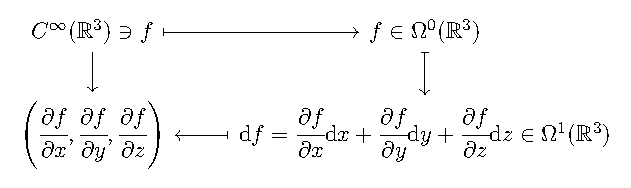
\includegraphics{lectures/7/pictures/cd_1.pdf}
		\end{center}	
		Он показывает, что композиция этих отождествленйи уже вполне каноническая (так как градиент функции не зависит от выбора координат). 

		Если же мы рассмотрим векторное $(f_1, f_2, f_3) = V$, изготовим из него $1$-форму, продифференцируем её и перегоним обратно в векторное поле, получится \emph{ротор} векторного поля $V$:
		\begin{center}
			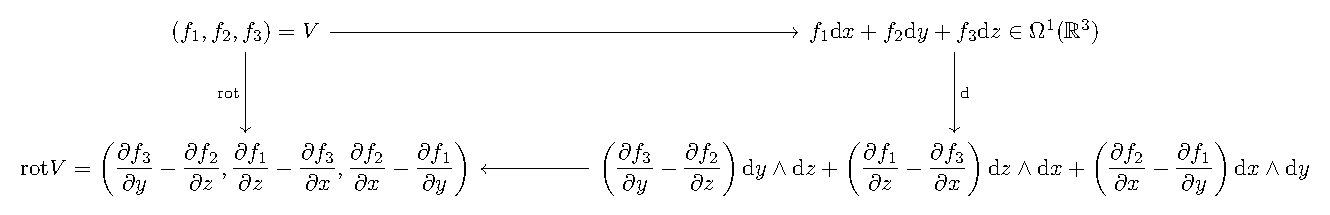
\includegraphics[scale = 0.8]{lectures/7/pictures/cd_44.pdf}
		\end{center}


		Аналогичное можно селать и с дивергенцией. 

		\begin{center}
			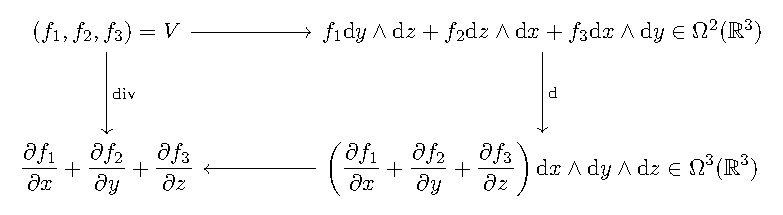
\includegraphics{lectures/7/pictures/cd_45.pdf}
		\end{center}

		То есть, мы только что поняли, что 
		\begin{itemize}
			\item $\mathrm{d}(0$-формы) = градиент, 
			\item $\mathrm{d}(1$-формы) = ротор,
			\item $\mathrm{d}(2$-формы) = дивергенция,
		\end{itemize}

		К слову, отсюда мы бесплатно получили вот такие свойство: 
		\[
			\rot{\nabla f} = 0, \quad \Div{\rot{V}} = 0.
		\]
	\end{example}



	






	


